\documentclass[10pt]{beamer}

\usepackage{amsmath}
\usepackage{amssymb}
\usepackage{booktabs}
\usetheme{Warsaw}


\title{K-Means, K-Center, and KNN}
% \subtitle{A modern beamer theme}
\date{\today}
\author{John Ensley, Mohammed Mottahedi \& Songshan Yang}
\institute{Penn State University \\ STAT 557}
\titlegraphic{\hfill
\includegraphics[height=1.75cm]{psulogo}}

\begin{document}

\maketitle

\begin{frame}\frametitle{Data Description}
\begin{itemize}
  \item 699 tumor samples
  \item 458 classified as benign, 241 as malignant
  \item 9 observations for each: uniformity of cell size, uniformity of cell shape, marginal adhesion, single epithelial cell size, bare nuclei, bland chromatin, normal nucleoli, mitoses
  \item Each predictor is a value from 1 to 10
\end{itemize}
\end{frame}

\begin{frame}\frametitle{K-Means}
    Implemented in two ways:
    \begin{itemize}
        \item Split data set randomly into 50\% training, 50\% test
        \item 5-fold cross validation
    \end{itemize}

    Compared error rates over varying number of prototypes

    \begin{center}
    \begin{tabular}{rcccccc}
        \toprule
        Number of prototypes & 1 & 2 & 3 & 4 & 5 & 6 \\
        \midrule
        Error rates, training set & 0.35 & 0.0453 & 0.086 & 0.135 & 0.205 & 0.234 \\
        Error rates, 5-fold CV & 0.35 & 0.0424 & 0.083 & 0.116 & 0.213 & 0.227 \\
        \bottomrule
    \end{tabular}
    \end{center}
\end{frame}

\begin{frame}\frametitle{K-Means}
    \begin{center}
        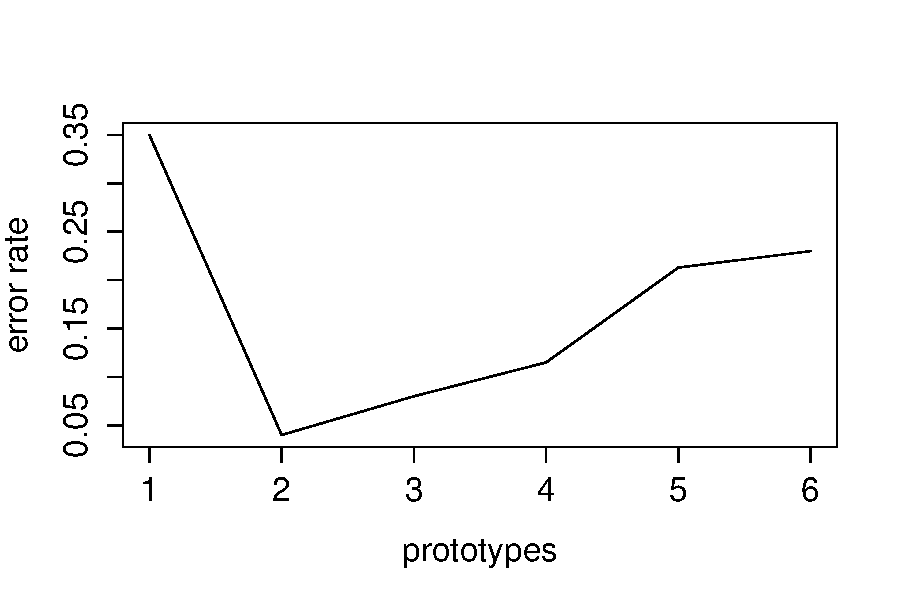
\includegraphics[width=0.7\textwidth]{1.pdf}
    \end{center}

    Optimal number of prototypes is 2.
\end{frame}

\begin{frame}\frametitle{K-Means with Dimension Reduction}
    Used first two principal components, accounting for 74\% of the total variance. Again 2 prototypes optimal. Classification is not improved with this data.

    \begin{center}
    \begin{tabular}{rcccccc}
        \toprule
        Number of prototypes & 1 & 2 & 3 & 4 & 5 & 6 \\
        \midrule
        Error rates, 2 PCs & 0.35 & 0.041 & 0.146 & 0.202 & 0.2225 & 0.197 \\
        \bottomrule
    \end{tabular}

    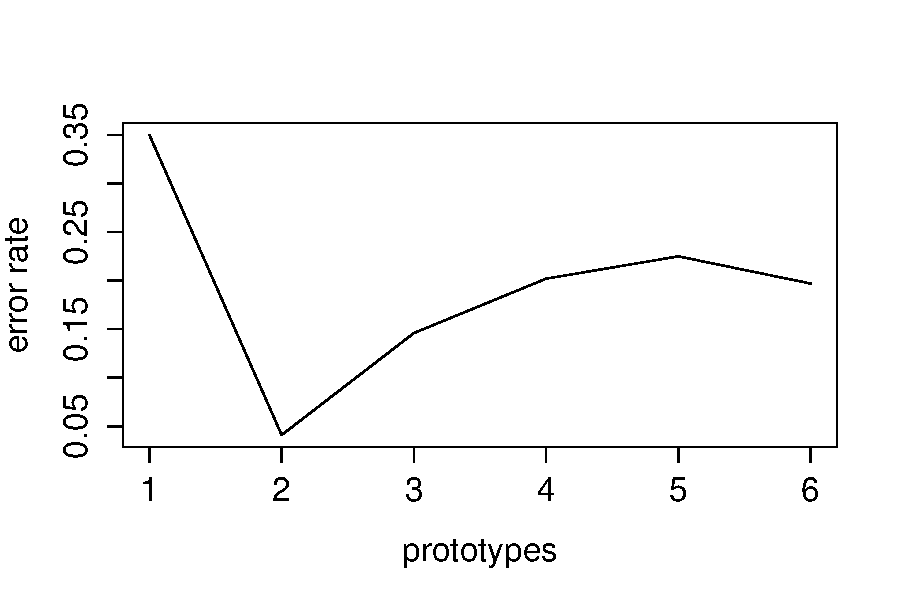
\includegraphics[width=0.65\textwidth]{7.pdf}
    \end{center}
\end{frame}

\begin{frame}\frametitle{K-Nearest Neighbor}
    Implemented in two ways:
    \begin{itemize}
        \item Split data set randomly into 50\% training, 50\% test
        \item Leave-one-out cross validation
    \end{itemize}

    Compared error rates across different values of $k$

    \begin{center}
        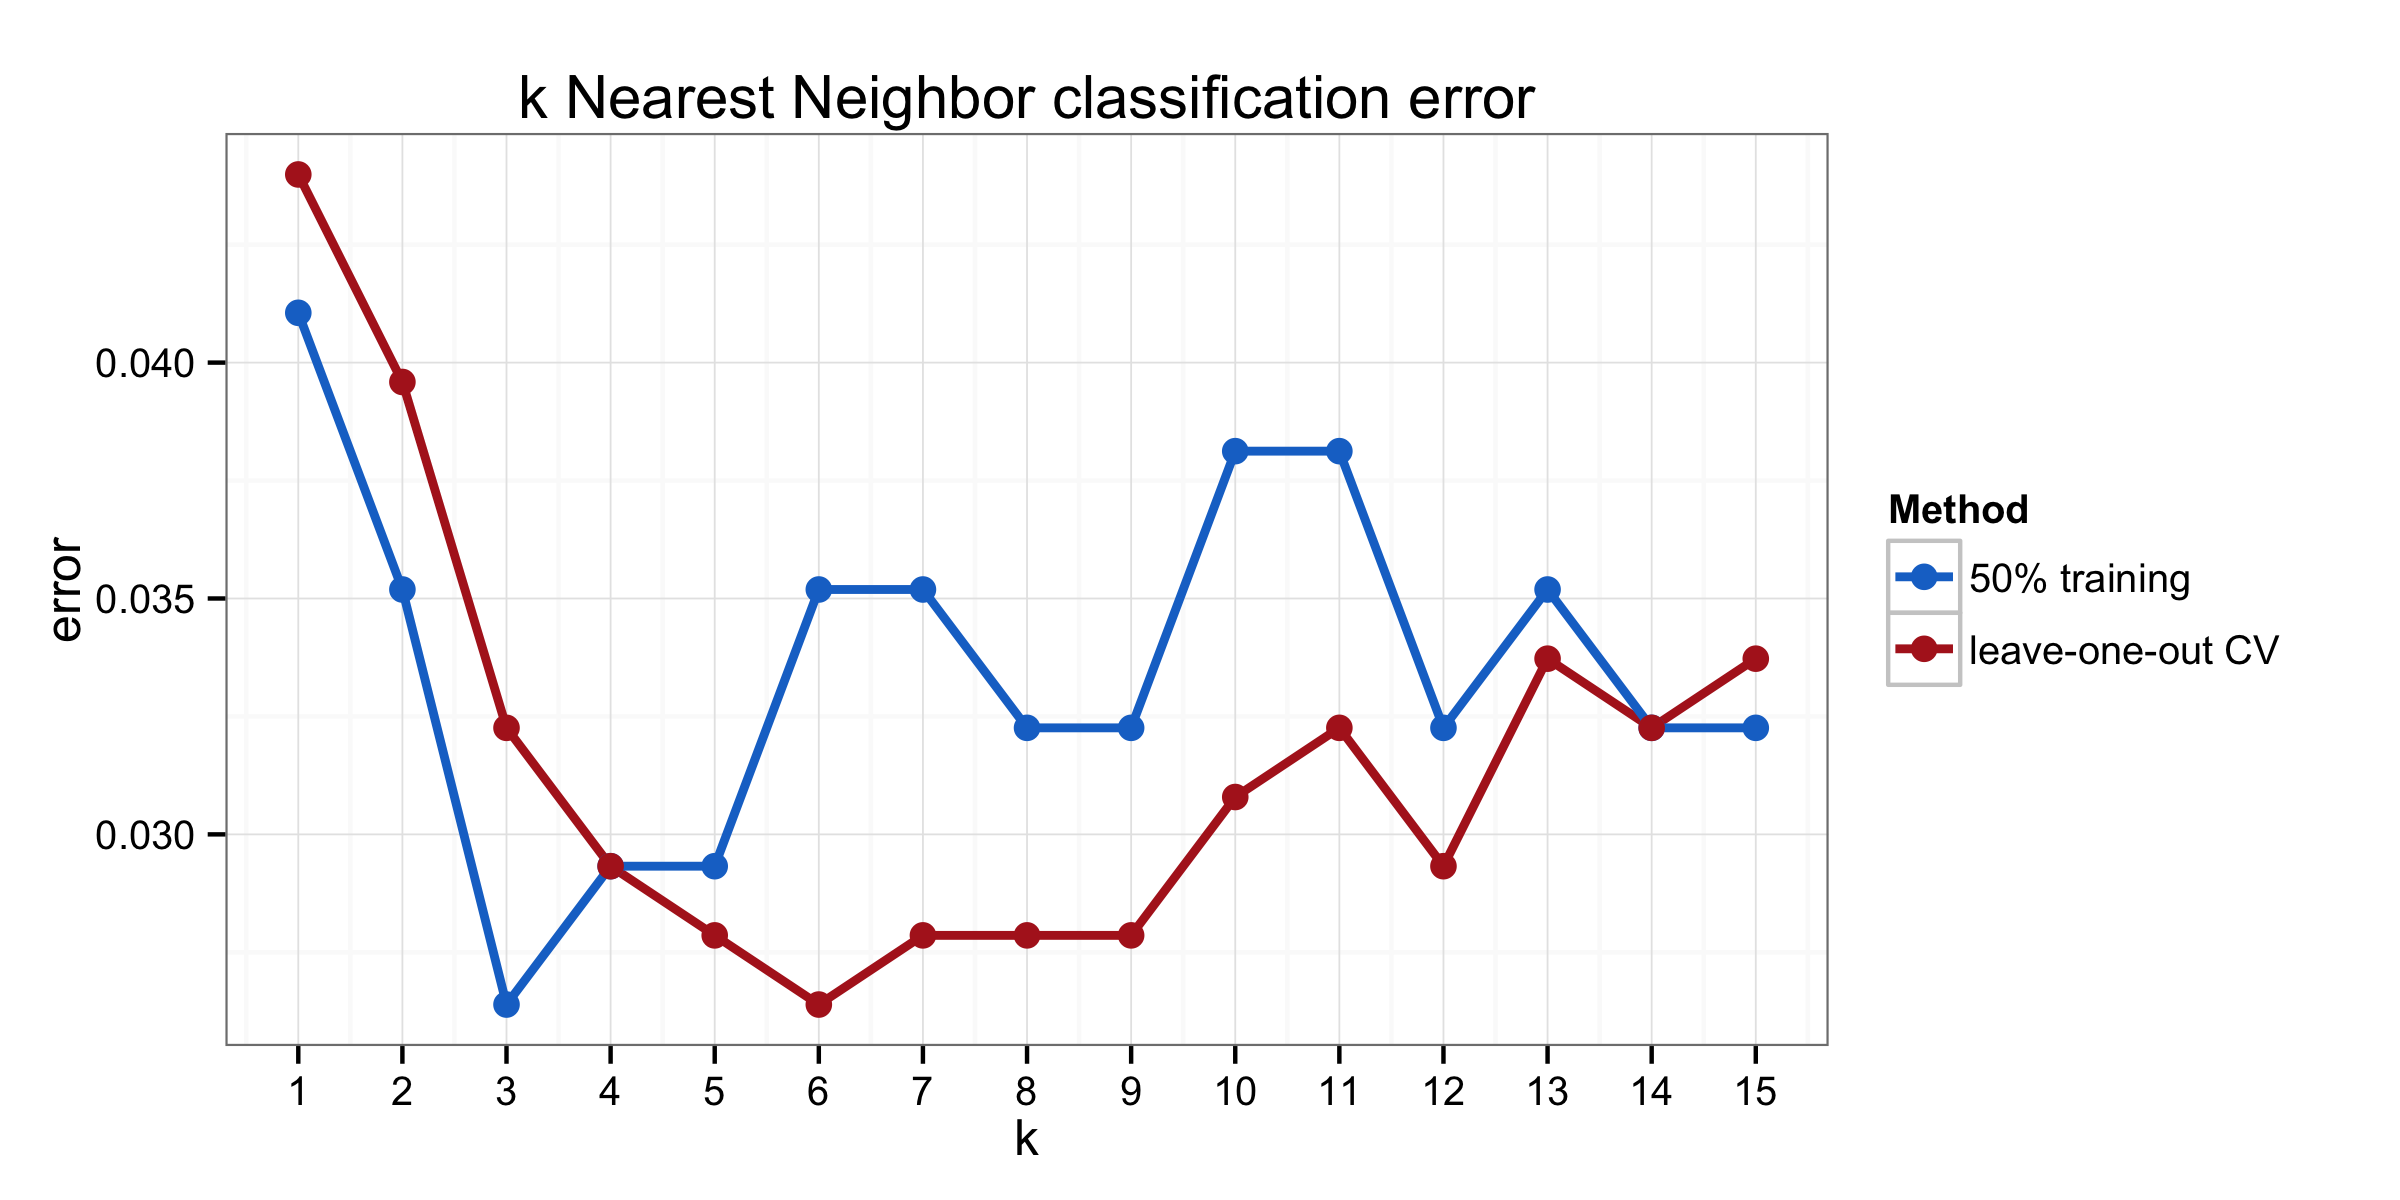
\includegraphics[width=\textwidth]{knn1.png}
    \end{center}
\end{frame}

\begin{frame}\frametitle{Unsupervised Clustering}
    \framesubtitle{K-means}
     Without considering class labels we try several different numbers of clusters ($2-6$) for the data set.
    \begin{figure}
        \centering
        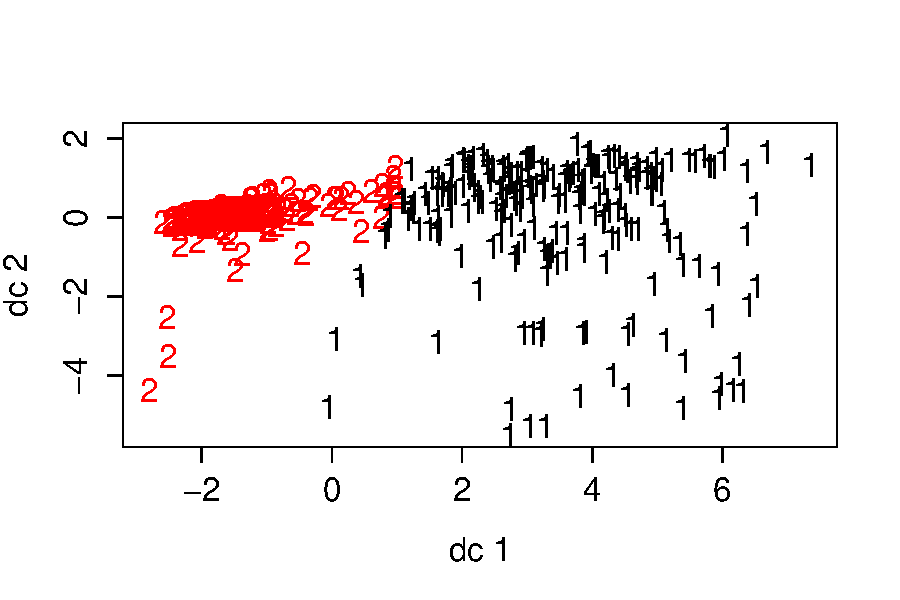
\includegraphics[width=0.5\textwidth]{2.pdf}
        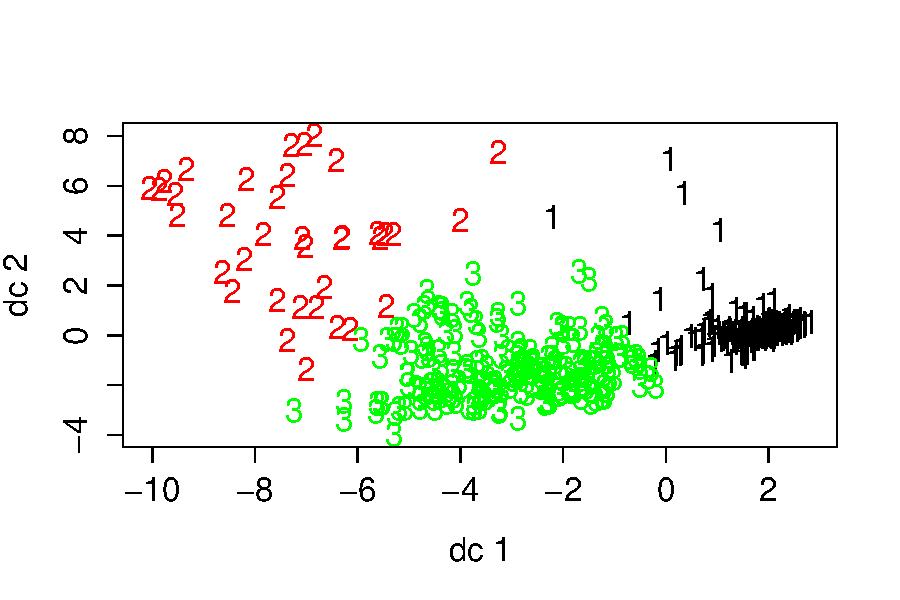
\includegraphics[width=0.5\textwidth]{3.pdf}
        \end{figure}

\end{frame}

  \begin{frame}
    \frametitle{Unsupervised Clustering}
    \framesubtitle{K-means}

    \begin{figure}
    \centering
    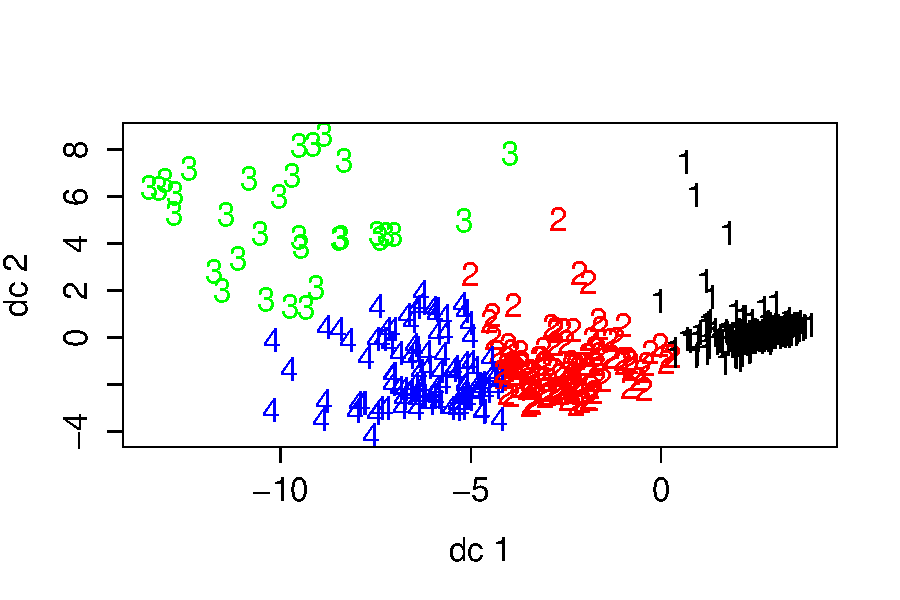
\includegraphics[width=0.5\textwidth]{4.pdf}
    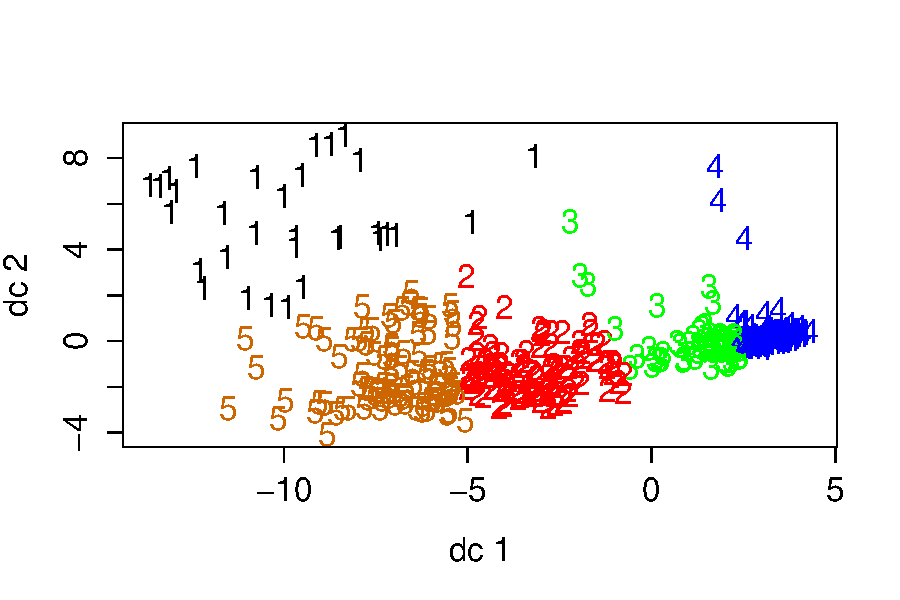
\includegraphics[width=0.5\textwidth]{5.pdf}
    \end{figure}

    \begin{figure}
    \centering
    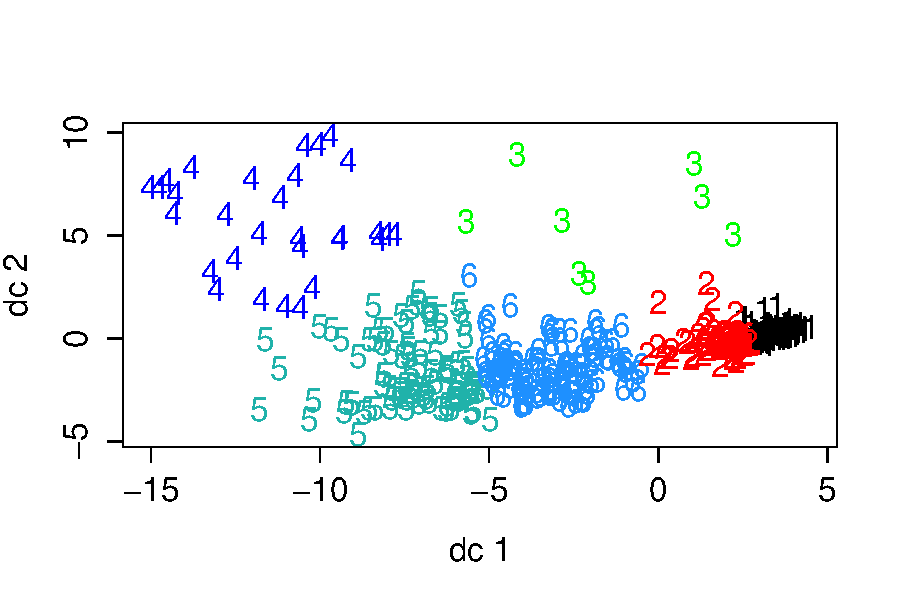
\includegraphics[width=0.5\textwidth]{6.pdf}
    \caption{K-means unsupervised clustering results}
    \end{figure}
    \end{frame}


  \begin{frame}
    \frametitle{Unsupervised Clustering}
    \framesubtitle{K-centers}
    We try to minimize the maximum inter-cluster distance.
    Ignoring class labels:
    \begin{figure}
    \centering
    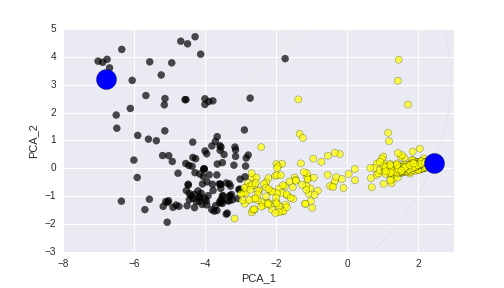
\includegraphics[width=0.5\textwidth]{m1.png}
    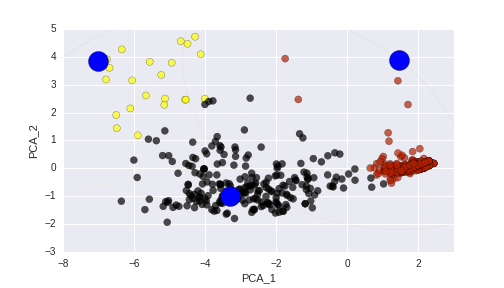
\includegraphics[width=0.5\textwidth]{m2.png}
    \caption{K-center unsupervised clustering results}
    \end{figure}


    \end{frame}

  \begin{frame}
    \frametitle{Unsupervised Clustering}
    \framesubtitle{K-centers}

    \begin{figure}
    \centering
    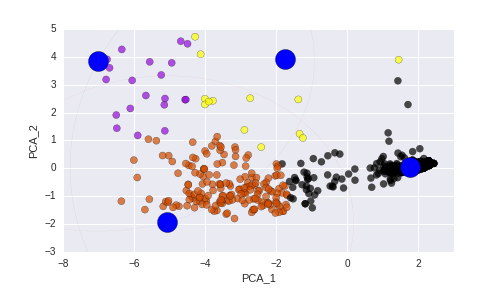
\includegraphics[width=0.5\textwidth]{m3.png}
    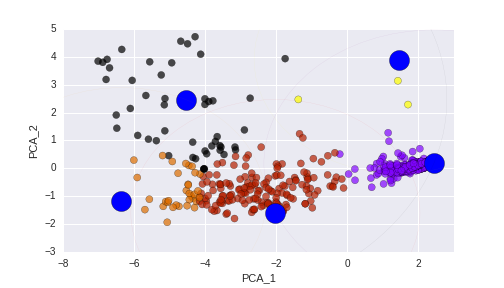
\includegraphics[width=0.5\textwidth]{m4.png}
    \end{figure}

    \begin{figure}
    \centering
    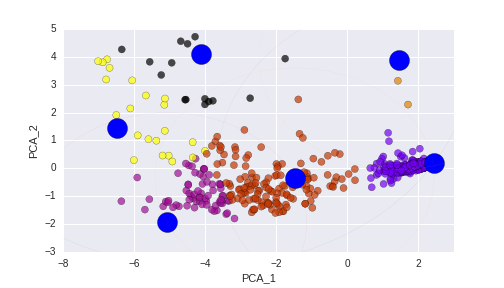
\includegraphics[width=0.5\textwidth]{m5.png}
    \caption{K-center unsupervised clustering results}
    \end{figure}

    \end{frame}

    \begin{frame}
    \frametitle{Unsupervised Clustering}
    \framesubtitle{k-means vs k-centers}

    K-center focuses on worst case scenario and k-means focuses on average distance.

    \begin{figure}
    \centering
    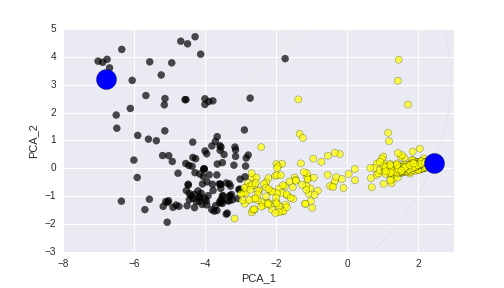
\includegraphics[width=0.5\textwidth]{m1.png}
    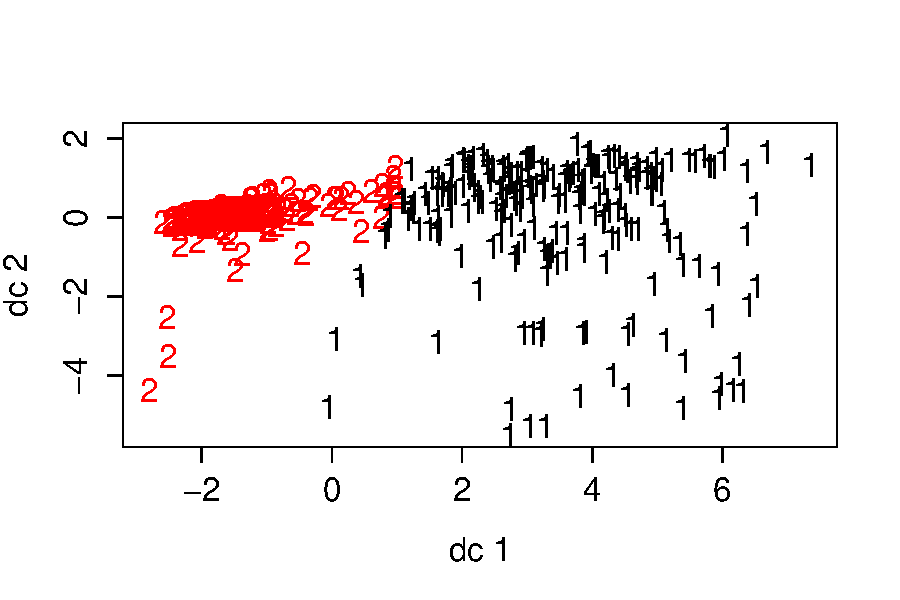
\includegraphics[width=0.5\textwidth]{2.pdf}
    \end{figure}

    \end{frame}


    \begin{frame}
    \begin{center}
    \Large
    Questions?
    \end{center}

    \end{frame}

\end{document}